\section{Interaction Engineering - Fragenkatalog}
\subsection{Introduction}
\begin{enumerate}
	\item Erkläre Stärken und Schwächen des Menschens und des Computers in der Human-Computer Interaction!
	\begin{table}[!h]
		\centering
		\begin{tabular}{|p{20em}|p{20em}|}
			\hline
			Mensch & Computer\\
			\hline
			\tabitem Kreativität & \tabitem 'exakte'\footnote{Denke an max. Genauigkeit von Fließkommazahlen!} Berechnungen\\
			\tabitem Abstrahieren und Erzeugen von Modellen & \tabitem stundenlanges Ausführen derselben Aufgabe ohne zu Ermüden\\
			\tabitem auf Unerwartetes reagieren& \tabitem exakter Speicher (Gedächtnis)\\
			\hline
		\end{tabular}
		\caption{Stärken des Menschen und Computers in HCI. (Särken = Schwächen des anderen!)}
		\label{strength_of_hc}
	\end{table}
	
	\item Kernunterschied bei der Entwicklung von computional solutions und interactive solutions
	\begin{itemize}
		\item Interaction: Kernfaktor ist das Human Computer Interface
		\item Computational: Kern ist effizienter Algorithmus(?)
		\item Rechenleistung steigt immer weiter während menschliche Aufnahmefähigkeit stagniert/konstant ist
		\item Kernfaktor bei der Informationsverarbeitung durch den Menschen ist das Interface
		\item $\Rightarrow$ Interaction soll smooth und effizient; Feedback soll reich an Informationen und instantan sein
		\item HC-Interaction - Mensch und Computer gehen Hand in Hand, jeder erfüllt die Aufgaben, die er am besten lösen kann (siehe Tabelle \ref{strength_of_hc})
		\begin{table}[!h]
			\centering
			\begin{tabular}{|l|l|}
				\hline
				\textbf{Computation} - closed system & \textbf{Interaction} - open system\\
				\hline
				\tabitem Eingabe & \tabitem Veränderung in der Umwelt\\
				\tabitem Verarbeitung & \tabitem Empfange Events\\
				\tabitem Ausgabe  & \tabitem Reagiere auf Events\\
				\tabitem deterministisch, Endzustand & \tabitem endlos, nichtdeterministisch\\
				\hline
			\end{tabular}
		\end{table}
	\end{itemize}
	
	\item Action Cycle by Norman
	\begin{enumerate}
		\item Mensch hat Ziel im Kopf (Goal)
		\item Planen der notwendigen Schritte (Plan)
		\item Spezifizieren der Schritte (Specify) 
		\item Umsetzen der Schritte in der Welt (Perform)
		\item Feedback in der Welt beobachten (Perceive) 
		\item Feedback interpretieren (Interpret)
		\item Ergebnis mit Zielen vergleichen (Compare)
		\item Beginne bei Schritt 1 bzw. 2
	\end{enumerate}
	\begin{figure}[!h]
		\centering
		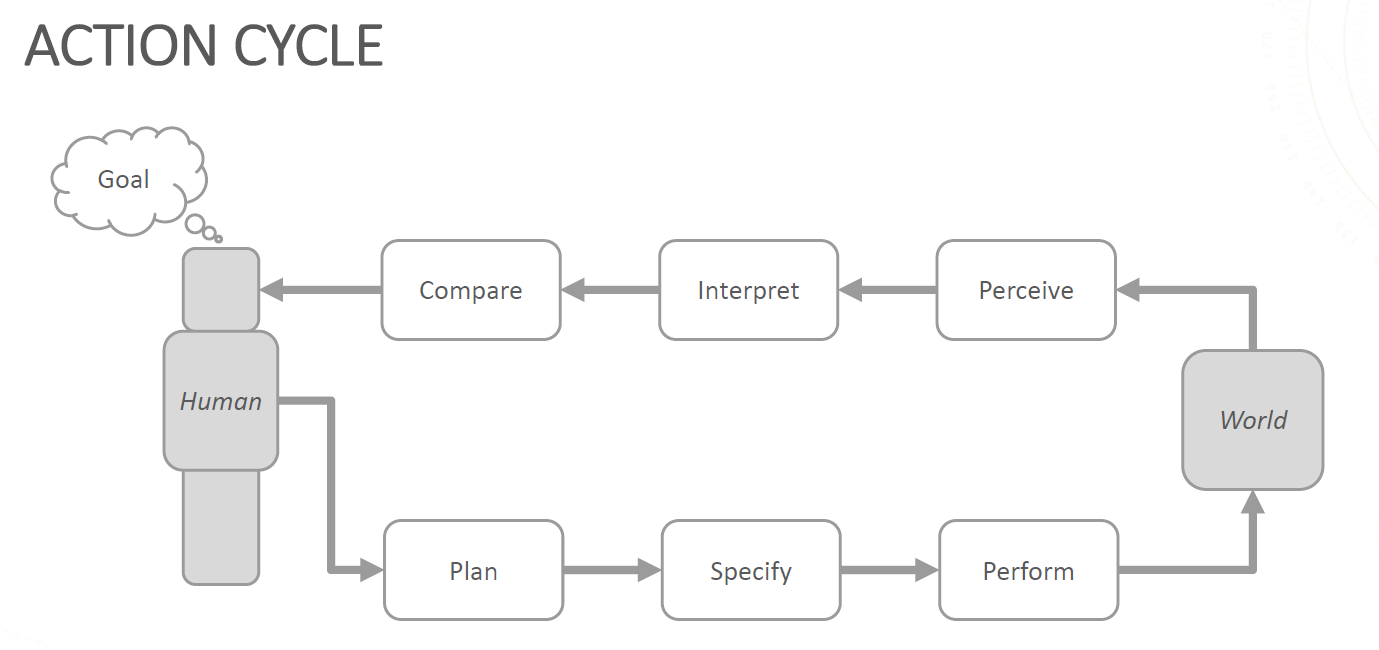
\includegraphics[scale=0.4]{img/action_cycle.png}
		\caption{Action Cylce nach Norman}
	\end{figure}
	
	\item Iteration/Bsp für den Action Cycle\\
	Am Beispiel: Kaffee holen in der Mensa
	\begin{itemize}
		\item \textbf{Goal:} Kaffee in der Mensa holen
		\item \textbf{Plan:} Aus dem Büro gehen
		\item \textbf{Specify:} Operation - Türgriff betätigen um Bürotür zu öffnen
		\item \textbf{Perform:} Türgriff drücken
		\item \textbf{Perceive:} Griff öffnet das Schloss, Tür öffnet sich
		\item \textbf{Interpret:} Tür ist offen
		\item \textbf{Compare:} Schritt erfolgreich, Führe weitere Schritte aus
	\end{itemize}
	
	
	\item  Gulf of Execution and Evalutation
	\begin{itemize}
		\item \textbf{Execution}\\
		beschreibt die Mühe/Aufwand der angestrebten Aufgaben\\
		Kann ich das tun? Wo ist die notwendige Funktionalität? Welches Gerät nutze ich? Wie führe ich das Kommando aus?
		\item \textbf{Evaluation}\\
		Beschreibt die Mühe/Aufwand die Veränderung der Umwelt zu interpretieren\\
		Ist überhaupt etwas passiert? Wo ist etwas passiert? Was ist passiert? Passen Effekt und Absicht zusammen?
		\item Interaction cost = Summe des physischen und mentalen Aufwandes um ein Ziel zu erreichen
		\item Beispielhaft am Action Cycle:
		\begin{itemize}
			\item Cost of Decision (Goal): Fokus muss auf Teilmenge von Informationen und Interfaces gelenkt werden
			\item Cost of System Power (Plan): Übersetzen von Zielen im Kopf in Operationssequenzen ist schwer, insbesondere für komplexe Systeme
			\item Cost of visual clutter/visuelle Überfuütung/reizung (Perceive): Bsp - Mouse Hover Effekte erzeugen Überreizung und erschweren Zustandswahrnehmung 
		\end{itemize}
	\end{itemize}
	
	\item The Three levels of interaction
	\begin{itemize}
		\item \textbf{low level:} Selection and Manipulation
		\item \textbf{inter-mediate level:} Exploration and Navigation
		\item \textbf{high level:} Problem-solving
	\end{itemize}
	
	\item The levels of (human) interaction processing
	\begin{itemize}
		\item Instinktiv (Perform and Perceive): vollkommen unterbewusst, ohne Kontrolle, schnell, Basisfähigkeiten - Bsp: Arm bewegen um Türgriff zu fassen
		\item Behavioral (Specify and Interpret): teilweise unterbewusst, leichte Kontrolle, schnell, gelernte Fähigkeiten - Bsp: Drücken der Klinke öffnet Tür
		\item Reflective (Plan and Compare): volles Bewusstsein, langsam, komplexe Analyse - Bsp: Tür ist offen, was bedeutet das?
	\end{itemize}
	
	\item at least 5 golden rules or guidelines for interaction\\
	\textbf{Golden Rules - Norman}
	\begin{enumerate}
		\item Discoverability: Welche (möglichen) Aktionen können bestimmt werden?
		\item Feedback: reichhaltiger und kontinuierlicher Fluss an Informationen über den Zustand
		\item Affordances: angemessene Aufforderungen um die gewünschte Aktion durchzuführen
		\item Signifiers: effiziente Signalgeber für Discoverability und Feedback
		\item Mappings: gute Zuordnung zwischen Controls and Actions
	\end{enumerate}
	\textbf{Guidelines - Shneiderman}
	\begin{enumerate}
		\item Konsistenz: ähnliche Situationen sollen ähnliche Aktionen erfordern
		\item Universal Usability: Assistenz anbieten (Hilfe, Shortcuts,..)
		\item Informative Feedback: Feedback für jede Useraktion
		\item Closure: klarer Beginn, Ablauf und Ende einer Aktion; kombiniere mit Punkt 3
		\item Prevent Error: vermeide fehlerhaften input, Recover from user error
		\item Easy reversal of actions: zb undo redo
		\item internal locus of control: User kontrolliert das System
		\item reduce short-term memory load: keep it simple
	\end{enumerate}
\end{enumerate}

\textbf{Sonstige Notizen}
\begin{itemize}
	\item Vor- und Nachteile der Interaction
	\begin{table}[!h]
		\centering
		\begin{tabular}{|p{20em}|p{20em}|}
			\hline
			\textbf{Vorteile} & \textbf{Nachteile}\\
			\hline
			\tabitem ist mächtiger als ''Algorithmen'' & \tabitem User muss wissen \textit{was} er/sie möchte\\
			\tabitem anspruchsvolleres Verhalten & \tabitem User muss wissen \textit{wie} er/sie den Computer bedienen muss um das Ziel zu erreichen\\
			 & \tabitem Anwendung ist zustandsbehaftet -> User kann sich verlieren/steckenbleiben (stateful things can be broken)\\
			\hline
		\end{tabular}
	\end{table}
	
	\item Bottlenecks - Processing: CPU, RAM, Netzwerk etc.. mittlerweile in vielen Anwendungsgebieten nicht mehr so relevant
	\item Bottlenecks - Information: enorm wichtig welche Daten auf dem kleinen Bildschirm am Ende angezeigt werden (viele, viele Daten gespeichert; welche Davon sind wichtig und werden angezeigt?)
	\item Bottlenecks - Aufnahmefähigkeit Mensch
\end{itemize}